\documentclass[border=10pt]{standalone}
%%%<
\usepackage{verbatim}
%%%>
\usepackage{pgfplots}
\pgfplotsset{width=7cm,compat=1.8}
\begin{comment}
:Title: Bar plot
:Tags: 2D;Bar plots;Manual
:Author: Christian Feuersänger
:Slug: bar-plot

Bar plots place horizontal or vertical bars at coordinates. Multiple bar plots
in one axis can be stacked on top of each other or aligned next to each other.

The code is from the PGFPlots 1.10 manual: "4.5.4 Bar Plots".
\end{comment}
\begin{document}
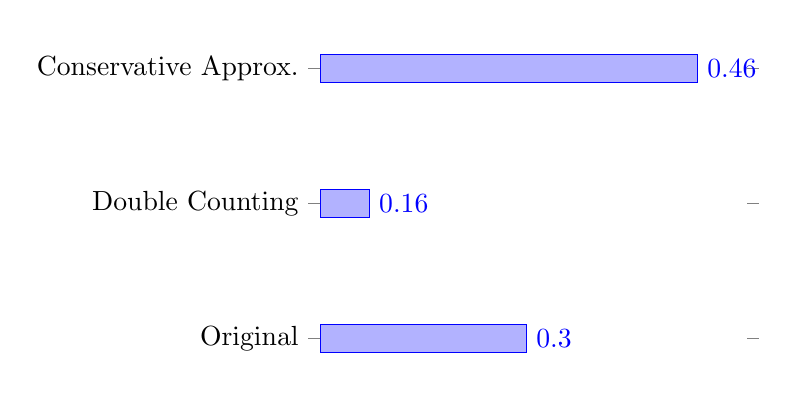
\begin{tikzpicture}
\begin{axis}[
    xbar,
    y axis line style = { opacity = 0 },
    axis x line       = none,
    enlargelimits=0.15,
    symbolic y coords={Original,Double Counting,Conservative Approx.},
    xtick=data,
    nodes near coords
    ]
    
\addplot coordinates { (0.3,Original)   (0.1552,Double Counting) (0.4577,Conservative Approx.)   };
%\addplot coordinates { (0.7,Original)   (0.8448,Double Counting) (0.5423,Conservative Approx.)   };
      
%\addplot coordinates { (Original,0.3)   (Double Counting, 0.1552) (Conservative Approx.,0.4577)   };
%\addplot coordinates { (Original,0.7)   (Double Counting, 0.8448) (Conservative Approx., 0.5423)   };
%      
      
%      
%\addplot coordinates {(tool8,7) (tool9,9) (tool10,4)};
%\addplot coordinates {(tool8,4) (tool9,4) (tool10,4)};
%\addplot coordinates {(tool8,1) (tool9,1) (tool10,1)};
\end{axis}
\end{tikzpicture}
\end{document}